\documentclass[english]{achemso}
\setkeys{acs}{keywords = true, email=false}
\usepackage[T2A,LGR,T1]{fontenc}
\usepackage{babel}
\usepackage{array}
\usepackage{textcomp}
\usepackage{url}
\usepackage{multirow}
\usepackage{amsmath}
\usepackage{graphicx}
\usepackage{subscript}
%\usepackage[bottom]{footmisc}
%\usepackage[unicode=true,pdfusetitle,
% bookmarks=true,bookmarksnumbered=false,bookmarksopen=false,
% breaklinks=false,pdfborder={0 0 0},pdfborderstyle={},backref=false,colorlinks=false]
% {hyperref}
%\usepackage{lineno}
%\linenumbers

\makeatletter

%%%%%%%%%%%%%%%%%%%%%%%%%%%%%% LyX specific LaTeX commands.


\title{Wetting of the tarsal adhesive fluid determines underwater adhesion in ladybug beetles: Supplementary information}

\author{Pranav Sudersan}


\affiliation{Max Planck Institute for Polymer Research, Ackermannweg 10, 55128
Mainz, Germany}


\author{Michael Kappl}


\affiliation{Max Planck Institute for Polymer Research, Ackermannweg 10, 55128
Mainz, Germany}


\author{Bat-El Pinchasik}


\affiliation{School of Mechanical Engineering, Tel Aviv University, Tel Aviv-Yafo,
Israel}


\author{Hans-J\"{u}rgen Butt}


\affiliation{Max Planck Institute for Polymer Research, Ackermannweg 10, 55128
Mainz, Germany}


\author{Thomas Endlein}


\affiliation{Max Planck Institute for Polymer Research, Ackermannweg 10, 55128
Mainz, Germany}


\DeclareRobustCommand{\greektext}{%
  \fontencoding{LGR}\selectfont\def\encodingdefault{LGR}}
\DeclareRobustCommand{\textgreek}[1]{\leavevmode{\greektext #1}}
\ProvideTextCommand{\~}{LGR}[1]{\char126#1}

\DeclareRobustCommand{\cyrtext}{%
  \fontencoding{T2A}\selectfont\def\encodingdefault{T2A}}
\DeclareRobustCommand{\textcyr}[1]{\leavevmode{\cyrtext #1}}

\newcommand{\lyxmathsym}[1]{\ifmmode\begingroup\def\b@ld{bold}
  \text{\ifx\math@version\b@ld\bfseries\fi#1}\endgroup\else#1\fi}

%% Because html converters don't know tabularnewline
\providecommand{\tabularnewline}{\\}

%%%%%%%%%%%%%%%%%%%%%%%%%%%%%% User specified LaTeX commands.
\SectionNumbersOn
%\setkeys{acs}{doi = true}
\setkeys{Gin}{width=\linewidth}
\usepackage{subcaption}
\usepackage[pagewise]{lineno}
\linenumbers

\makeatother

\begin{document}
%reset figure/table/equation numbers and include prefix
\renewcommand{\thesection}{S\arabic{section}}
\setcounter{figure}{0} \renewcommand{\thefigure}{S\arabic{figure}} 
\setcounter{table}{0} \renewcommand{\thetable}{S\arabic{table}} 
\setcounter{equation}{0} \renewcommand{\theequation}{S\arabic{equation}}

\section{Simulation method: Single capillary bridge \label{subsec:Simulation-Method}}

Capillary force due to a single adhesive fluid or bubble meniscus (termed ``capillary
bridge'') was calculated by performing simulations in Surface Evolver
\cite{RN206}, similar to the method described by \citet{RN93}.
A simple cubic geometry, mimicking the capillary bridge, of constant
volume, $V$, was defined as the initial condition with an interfacial
tension, $\gamma$, with the surrounding medium. Interfacial tension
of the capillary bridge with the substrate is given by $\gamma\cos\theta$,
where $\theta$ is the corresponding contact angle inside the bridge.
For the case of a bubble meniscus, $\theta$ is defined w.r.t. the
surrounding water, since $\theta$ can also directly characterise
the substrate wettability. The capillary bridge spans a gap distance
$d$ between the top face and the substrate. The boundary conditions
were set corresponding to a pinned contact line of diameter $D$ on
the top face and constant interfacial tension with the substrate on
the bottom. All lengths were normalised relative to length $s=\left(3V/4\pi\right)^{1/3}$.
An appropriate refinement and iteration routine was chosen by trial-and-error to get a stable converged solution corresponding to the minimum energy state of the capillary bridge surface. The normalised
total capillary force, $\hat{f}=f/\gamma s$, is the sum of the Laplace
pressure and surface tension contributions , where:

\begin{equation}
f=f_{laplace}+f_{surface\,tension}=\varDelta P_{laplace}A_{_{bottom}}+2\pi R_{bottom}\gamma\sin\theta\label{eq:f_bridge}
\end{equation}

Here, $\varDelta P_{laplace}$ is the Laplace pressure of the equilibrium
capillary bridge, $A_{bottom}$ is the contact area of the capillary
bridge with the substrate at bottom and $R_{bottom}$ is the corresponding
radius of contact, all obtained from the simulation output for the
equilibrium surface.

The gap distance $d$ was varied stepwise and the capillary force was
calculated each time to obtain force-distance curves for a particular
choice of $D$ and $\theta$. 

%\section{Single capillary bridge: Effect of volume}
%
%Surface Evolver simulation results showing the effect of volume on
%the maximum capillary force of a single fluid bridge. Since the fluid
%is pinned at the top to the same diameter, D, a smaller volume would
%result in high interfacial curvatures, which increases the capillary
%force due to the negative Laplace pressure. In this case, small contact
%angles lead to a greater increase in adhesion.
%
%\begin{figure}[H]
%
%\begin{centering}
%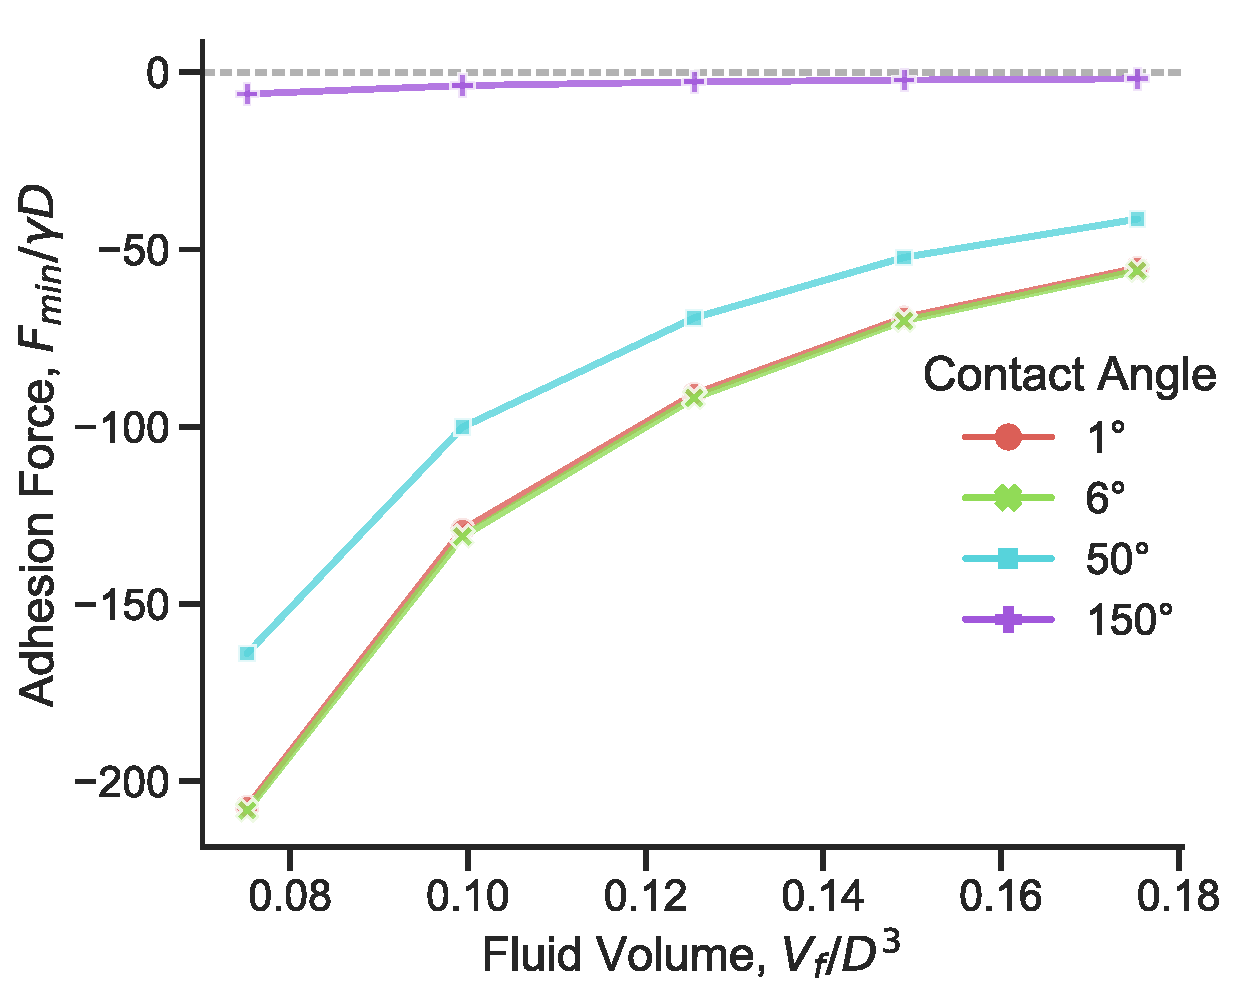
\includegraphics{FigureS2-Effect_of_fluid_volume}\caption{Normalised maximum capillary force for a single bridge as a function
%of fluid volume}
%\par\end{centering}
%\end{figure}
%
%
%\section{Capillary Bridge Model: Effect of hair diameter at constant fluid
%volume}
%
%Here, instead of scaling the fluid volume relative to the hair diameter,
%we now assume a fixed total fluid volume distributed equally among
%the $N$ hairs. Total fluid volume, $V_{total}=NV_{f}=2000$. Hair
%diameter is varied while keeping the total hair contact area constant.
%Length is in arbitrary units. Forces increase at a much smaller rate
%on decreasing diameter when compared to the case with self-similar
%scaling of fluid volume (Figure 8 in main text).
%
%\begin{figure}[H]
%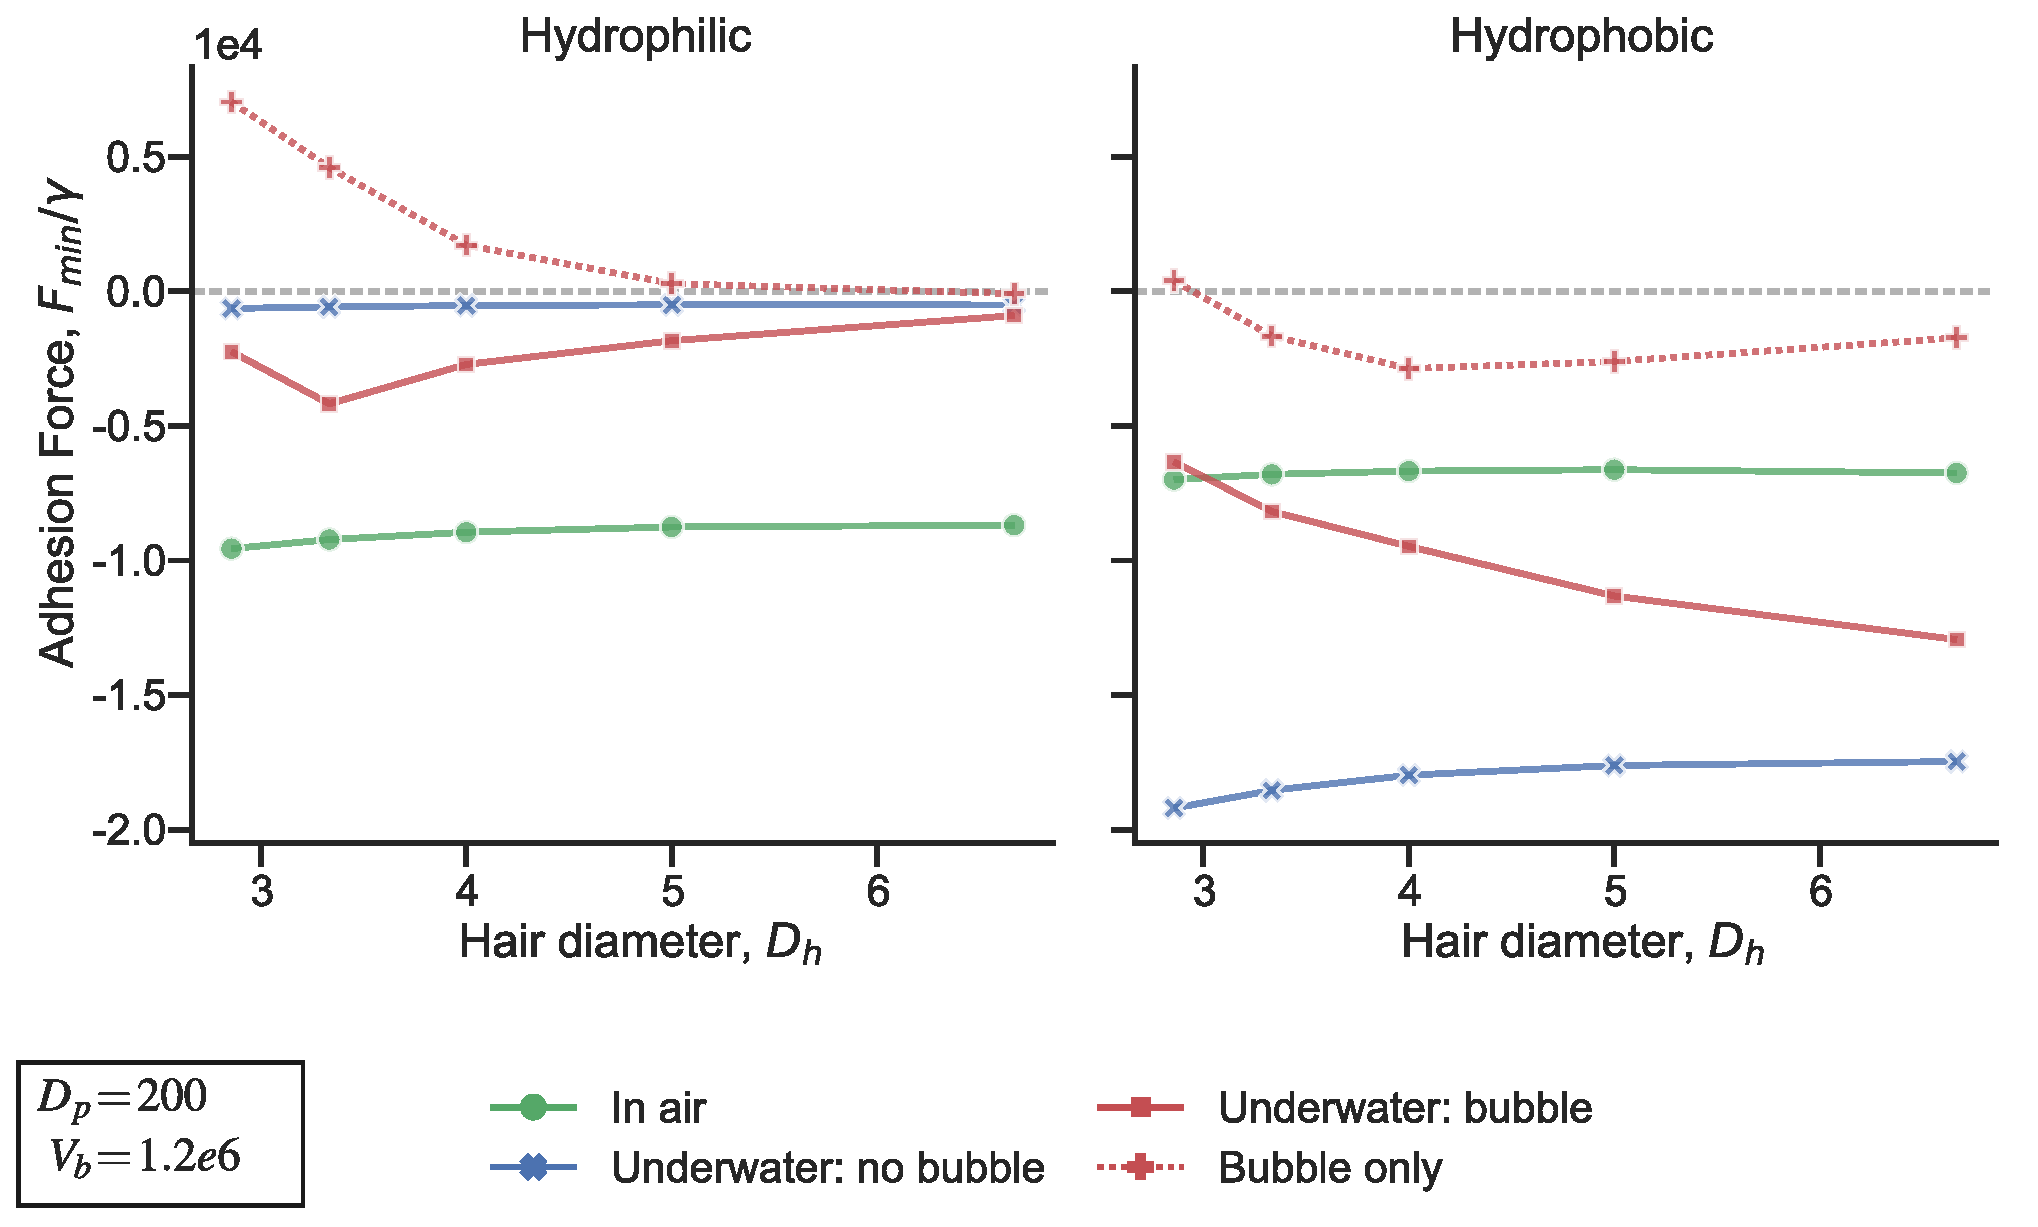
\includegraphics{FigureS3-Effect_of_hair_size(constant_vol)}
%
%\caption{Normalised adhesion force of hairy pad system on a hydrophilic and
%hydrophobic substrate as a function of hair diameter ($D_{h}$), calculated
%from the capillary bridge model. The total adhesive fluid volume is
%fixed to 2000. Adhesion forces are calculated from minima of the respective
%force-distance curves. Negative force value represents attraction.
%The bubble's contribution to the net force for an \emph{underwater:
%bubble} contact is denoted by plus symbols. Bubble volume and pad
%diameter are kept fixed. All lengths are scaled relative to $D_{p}$.}
%\end{figure}

\section{Substrate characterization}

The surface chemistry of untreated glass (hydrophilic) and PFOTS-coated glass (hydrophobic) was characterized using dynamic contact angle measurements (Table \ref{tab:Contact-Angles}). De-gassed water showed similar contact angle values as normal water.
\begin{table}[H]
\centering{}%
\begin{tabular}{|c|c|c|c|}
\hline 
Substrate & Liquid & \ensuremath{\theta}\textsubscript{A} & \ensuremath{\theta}\textsubscript{R}\tabularnewline
\hline 
\hline 
\multirow{2}{*}{Glass} & Water & 63\ensuremath{\pm}5\textdegree{} & 20\ensuremath{\pm}2\textdegree{}\tabularnewline
\cline{2-4} \cline{3-4} \cline{4-4} 
 & n-Hexadecane & <10\textdegree{} & <10\textdegree{}\tabularnewline
\hline 
\multirow{2}{*}{PFOTS} & Water & 122\ensuremath{\pm}1\textdegree{} & 93\ensuremath{\pm}2\textdegree{}\tabularnewline
\cline{2-4} \cline{3-4} \cline{4-4} 
 & n-Hexadecane & 88\ensuremath{\pm}2\textdegree{} & 56\ensuremath{\pm}5\textdegree{}\tabularnewline
\hline 
\end{tabular}\caption{Dynamic contact angles (Mean \ensuremath{\pm} SD, n = 3) of Milli-Q water and n-hexadecane on the different test substrates. \label{tab:Contact-Angles}}
\end{table}


\section{Statistical comparison}

Two-way ANOVA test showed a significant effect of the \emph{Contact mode} (p=0.001, F=9.596, degrees of freedom=2) 
and \emph{Substrate} (p<0.001, F=36.231, degrees of freedom=1) categories on the single leg adhesion force measurements
of the ladybug beetle (\emph{Coccinella septempuctata}). Signifanct interaction between the above two categories was seen (p=0.001, F=10.551, degrees of freedom=2). Post-hoc analysis results are shown below (Table \ref{tab:Statistical-analysis}).
The uncorrected p-values and Common Language Effect Size (CLES) were
obtained from pair-wise Student t-test between A and B while
keeping the third parameter fixed (degrees of freedom=8 for each pair). p-values showing statistically
significant difference between A and B are in boldface. 
CLES represents the statistical proportion of samples under A with higher adhesion than under B. The condition
for statistical significance is based on the Bonferroni-corrected
critical p-value of 0.008.

\begin{table}[H]
\noindent \begin{centering}
\begin{tabular}{|>{\raggedright}m{0.15\linewidth}|>{\raggedright}m{0.15\linewidth}|>{\raggedright}m{0.15\linewidth}||>{\centering}m{0.1\linewidth}|>{\centering}m{0.1\linewidth}|>{\centering}m{0.1\linewidth}|}
\hline
Fixed variable & A & B & T & p-value & CLES\tabularnewline
\hline 
\hline 
In air & PFOTS & Glass & -0.053 & 0.959 & 0.48\tabularnewline
\hline
Underwater: bubble & PFOTS & Glass & 3.292 & 0.011 & 0.96\tabularnewline
\hline
Underwater: no bubble & PFOTS & Glass & 10.044 & 0.0 & 1.0\tabularnewline
\hline
PFOTS & In air & Underwater: bubble & 0.133 & 0.897 & 0.48\tabularnewline
\hline
PFOTS & In air & Underwater: no bubble & -0.224 & 0.828 & 0.48\tabularnewline
\hline
PFOTS & Underwater: bubble & Underwater: no bubble & -0.37 & 0.721 & 0.44\tabularnewline
\hline
Glass & In air & Underwater: bubble & 4.688 & 0.002 & 1.0\tabularnewline
\hline
Glass & In air & Underwater: no bubble & 11.341 & 0.0 & 1.0\tabularnewline
\hline
Glass & Underwater: bubble & Underwater: no bubble & 2.086 & 0.07 & 0.84\tabularnewline
\hline 
\end{tabular}
\par\end{centering}
\caption{Post-hoc t-test results for each combination of contact mode and substrate\label{tab:Statistical-analysis}}
\end{table}

The effect of substrate, contact mode, tilt angle, beetle identity and repetition number on the adhesion were analysed using a linear mixed-effect model (LMEM) in Python. Here, each experimental data point was considered distinctly without averaging the repeats as before. Substrate, contact mode, tilt angle and repetition number were taken as fixed-effects, while, beetle identity was considered as the random-effect. Interaction between each of the fixed-effects were fitted using the random intercept model. Adhesion measurement on hydrophilic glass \emph{in air} was taken as the reference. The resultant fixed-effects coefficient estimates, standard error, z-statistic and p-value are reported below (Table \ref{tab:LMEM-analysis}). The random-effect (beetle identity) showed an intercept standard deviation of 100.563 \textmu N (std. error = 109.771)

\begin{table}[]
\begin{tabular}{|c|l|l|l|l|}
\hline
\multicolumn{1}{|l|}{}           & \multicolumn{1}{c|}{\textbf{Estimate}} & \multicolumn{1}{c|}{\textbf{Std. Error}} & \multicolumn{1}{c|}{\textbf{z}} & \multicolumn{1}{c|}{\textbf{p-value}} \\ \hline \hline
\textbf{Intercept \footnotemark[1]}               & 582.072                                & 170.307                                  & 3.418                           & 0.001                                 \\ \hline
\textbf{PFOTS}                   & -110.642                               & 206.268                                  & -0.536                          & 0.592                                 \\ \hline
\textbf{Underwater:   bubble}    & -304.667                               & 89.458                                   & -3.406                          & 0.001                                 \\ \hline
\textbf{Underwater: no   bubble} & -254.924                               & 117.386                                  & -2.172                          & 0.03                                  \\ \hline
\textbf{Repetition   number}     & 7.723                                  & 6.703                                    & 1.152                           & 0.249                                 \\ \hline
\textbf{Tilt angle}              & -5.649                                 & 7.088                                    & -0.797                          & 0.425                                 \\ \hline
\end{tabular}
\caption{Linear mixed-effect model statistics\label{tab:LMEM-analysis}}
\end{table}



\section{Capillary force due to an air bubble\label{subsec:Capillary-force-due}}

\footnotetext[1]{Adhesion on glass \emph{in air}}

Capillary force of a single air bubble against a PFOTS-coated glass surface are compared
for two different volumes (Figure \ref{fig:Bubble_capillary_force}). The volumes correspond to the expected
range for the case of the trapped air bubble in a ladybug's pad. Here, the bubble
was pinned to a micropatterned PDMS substrate on the top. Approach-retract tests were performed
at 62.5 \textmu m s\protect\textsuperscript{-1} speed. The maximum
adhesion force of any of the bubbles never exceeds 50 \textmu N,
significantly lower than the beetle's underwater adhesion to the same
substrate (> 400 \textmu N). Thus, the bubble's contribution
to adhesion in the ``\emph{underwater: bubble}'' contact of a ladybug's
pad should be negligible (< 10 \%). Example measurement video is included in the supplementary data (Movie3).

\begin{figure}[H]
\begin{centering}
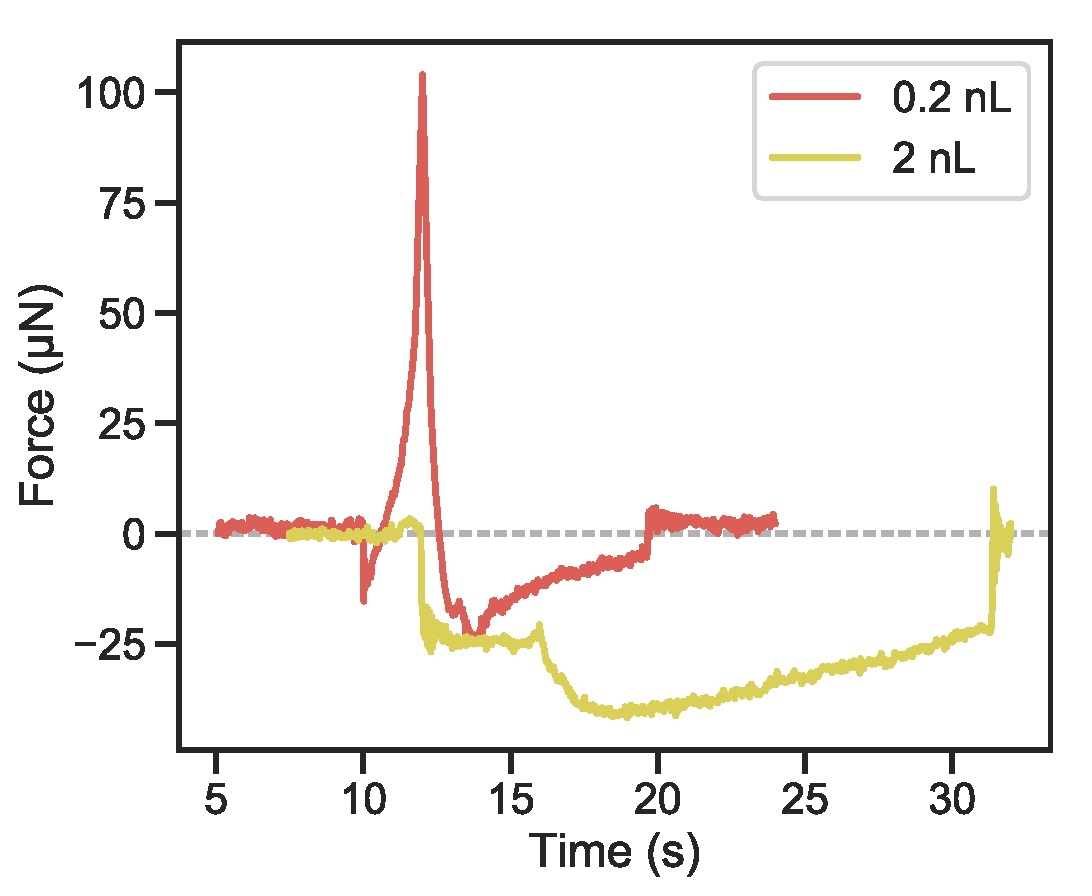
\includegraphics{FigureS4-Expt_bubble_force}\caption{Capillary force of the pinned bubble against a PFOTS-coated glass surface \label{fig:Bubble_capillary_force}}
\par\end{centering}
\end{figure}

\section{Capillary bridge model: Sensitivity analysis}

Sensitivity analysis was performed using the one-at-a-time (OAT) method. Dimensionless model parameters were initially set to correspond to the ladybug's case, as given by,
contact area fraction ($\alpha=ND_{h}^{2}/D_{p}^{2}=0.1$), pad to hair diameter ratio ($D_p/D_h=50$), hair aspect ratio ($L/D_{h}=10$), water surface tension ratio ($\gamma_{wa}/\gamma_{fa}=3$),
tarsal fluid-water interfacial tension ratio ($\gamma_{fw}/\gamma_{fa}=2$), tarsal fluid size parameter ($\phi_{f}=2$), bubble size parameter ($\phi_{b}=1.6$). Substrate contact angles were kept fixed (same as in main text). Each parameter was varied within a particular range, one at a time, and the corresponding adhesion forces \emph{in air} (F\textsubscript{a}),   \emph{underwater: no bubble} (F\textsubscript{w}) and \emph{underwater: bubble} (F\textsubscript{b}) were calculated. Linear least square regression was performed to quantify the relative change in adhesion for each contact mode with respect to the varied parameter. Here, F\textsubscript{w}/F\textsubscript{a} and F\textsubscript{b}/F\textsubscript{a} were taken to be the model output. Slope and R\textsuperscript{2} values for each case are reported below (Table \ref{tab:Sens-anal}). Slope with absolute values greater than 0.5 are highlighted in bold.


\begin{table}[H]
\begin{tabular}{|l|l|l|l|l|l|l|}
\hline
\multirow{2}{*}{\textbf{Parameter}} & \multirow{2}{*}{\textbf{Range}} & \multicolumn{1}{c|}{\multirow{2}{*}{\textbf{Substrate}}} & \multicolumn{2}{c|}{\textbf{F\textsubscript{w}/F\textsubscript{a}}}                                    & \multicolumn{2}{c|}{\textbf{F\textsubscript{b}/F\textsubscript{a}}}                                    \\ \cline{4-7} 
                                    &                                 & \multicolumn{1}{c|}{}                                    & \multicolumn{1}{c|}{\textbf{slope}} & \multicolumn{1}{c|}{\textbf{R\textsuperscript{2}}} & \multicolumn{1}{c|}{\textbf{slope}} & \multicolumn{1}{c|}{\textbf{R\textsuperscript{2}}} \\ \hline  \hline
\multirow{2}{*}{$\alpha$}              & \multirow{2}{*}{0.05 - 0.3}      & Hydrophilic                                              & 3.03E-18                                  & 1.52E-03                               & 2.30E-01                                  & 7.72E-01                               \\ \cline{3-7} 
                                    &                                 & Hydrophobic                                              & -9.69E-17                                 & 3.03E-03                               &\textbf{ -9.40E-01}                                 & 7.72E-01                               \\ \hline
\multirow{2}{*}{$D_p/D_h$}             & \multirow{2}{*}{30.0 - 60.0}     & Hydrophilic                                              & -8.83E-20                                 & 1.48E-01                               & 1.28E-02                                  & 9.73E-01                               \\ \cline{3-7} 
                                    &                                 & Hydrophobic                                              & -5.65E-18                                 & 1.48E-01                               & -1.51E-02                                 & 9.82E-01                               \\ \hline
\multirow{2}{*}{$L/D_{h}$}         & \multirow{2}{*}{8.0 - 15.0}      & Hydrophilic                                              & 0.00E+00                                  & 0.00E+00                               & -5.27E-02                                 & 9.11E-01                               \\ \cline{3-7} 
                                    &                                 & Hydrophobic                                              & 0.00E+00                                  & 0.00E+00                               & 5.41E-02                                  & 8.66E-01                               \\ \hline
\multirow{2}{*}{$\gamma_{wa}/\gamma_{fa}$}              & \multirow{2}{*}{2.5 - 3.5}       & Hydrophilic                                              & -2.01E-01                                 & 8.57E-01                               & -2.43E-01                                 & 9.43E-01                               \\ \cline{3-7} 
                                    &                                 & Hydrophobic                                              & 4.11E-02                                  & 1.00E+00                               & 6.87E-02                                  & 1.00E+00                               \\ \hline
\multirow{2}{*}{$\gamma_{fw}/\gamma_{fa}$}              & \multirow{2}{*}{1.5 - 2.5}       & Hydrophilic                                              & 2.01E-01                                  & 8.62E-01                               & 1.90E-01                                  & 8.94E-01                               \\ \cline{3-7} 
                                    &                                 & Hydrophobic                                              & \textbf{5.56E-01}                                  & 1.00E+00                               & 1.57E-01                                  & 1.00E+00                               \\ \hline
\multirow{2}{*}{$\phi_{f}$}             & \multirow{2}{*}{1.7 - 2.2}       & Hydrophilic                                              & 1.29E-02                                  & 4.52E-01                               & 6.18E-02                                  & 7.94E-02                               \\ \cline{3-7} 
                                    &                                 & Hydrophobic                                              & 7.67E-02                                  & 9.84E-01                               & -3.06E-01                                 & 9.66E-01                               \\ \hline
\multirow{2}{*}{$\phi_{b}$}             & \multirow{2}{*}{1.2 - 1.8}       & Hydrophilic                                              & 0.00E+00                                  & 0.00E+00                               & \textbf{-1.14E+00}                                 & 8.85E-01                               \\ \cline{3-7} 
                                    &                                 & Hydrophobic                                              & 0.00E+00                                  & 0.00E+00                               & \textbf{1.46E+00}                                  & 9.78E-01                               \\ \hline
\end{tabular}
\caption{Sensitivity analysis \label{tab:Sens-anal}}
\end{table}

\section{Supplementary video files}

\subsection*{Movie1}
Adhesion test recordings showing the three contact modes: \emph{in air},  \emph{underwater: bubble} and  \emph{underwater: no bubble} on a hydrophobic PFOTS-coated glass substrate. The two top panels of the video show the synchronous raw bottom-view and side-view recordings of the pad making contact with the substrate. The lower-left panel shows contact area extraction of the hairs with the surface via image processing and lower-right panel shows the corresponding temporal contact force and area data plot, with the data cursor synchronized with the other panels.

\subsection*{Movie2}
Adhesion test recording corresponding to the case of \emph{bad contact}, which occurred underwater on the PFOTS-coated glass substrate

\subsection*{Movie3}
Adhesion test recording of an air bubble (2nL volume) pinned to a microstructured PDMS on the top and making contact with a smooth PFOTS-coated glass substrate on the bottom.

\bibliography{references}

\end{document}